\addcontentsline{toc}{chapter}{Appendix}
\chapter*{Appendix A}
\renewcommand\thechapter{A}

\setcounter{section}{0} % Reset section counter


\newcommand{\customsection}[1]{%
    \refstepcounter{section}% Increment the section counter
    \section*{\thesection\quad #1}% Print the section with number, but don't add to ToC
}
\newcommand{\customsubsection}[1]{%
    \refstepcounter{subsection}% Increment the subsection counter
    \subsection*{\thesubsection\quad #1}% Print the subsection with number, but don't add to ToC
}


\customsection{Neural language models}\label{sec:LM} 
\customsubsection{Hyperparameters} \label{app:tm_training} 


\begin{table}
    \centering
    \scalebox{.9}{\begin{tabular}{lccccccc}
    \toprule
    & PPL & \# params & \# layers & lr & dropout  & tied layers & \makecell[c]{use positional\\ embedding}\\
    \midrule
    LSTM & 36.9$_{\pm 0.1}$ & 47.9M & 2 &  0.0001 & 0.1 &False& --\\
    $\mathcal{M}$ & 27.0$_{\pm 0.2}$ & 126.7M & 64 & 0.02 & 0.2 & False &True\\
    $\mathcal{M}_{shallow}$ & 37.8$_{\pm 0.7}$&49.5M & 2& 0.002& 0.0 &False& True\\
    $\mathcal{M}_{shared}$ &30.7$_{\pm 0.6}$ &47.8M &16 &0.002 &0.0  &True &True\\
    $\mathcal{M}_{nopos}$ & 27.4$_{\pm 0.3}$ &126.7M &16 &0.01 &0.1 &False &False\\
    \midrule
    MLM & $^\dagger$ 5.6$_{\pm 1.2}$ & 130.5M& 16 &0.02 & 0.2&False & True\\
    $\text{MLM}_{nopos}$ & $^\dagger$ 57.2$_{\pm 2.3}$ & 130.5M&16 &0.02 &0.2 & False& False\\
    \bottomrule
    \end{tabular}}
    \caption{Hyperparameter configurations for each model and their corresponding average perplexity scores. $^\dagger$ denotes pseudo-perplexity scores used for MLM evaluation (\S\ref{sec:exp_2_mlm_nopos}), not comparable with conventional perplexity scores.  }
    \label{tab:hyper}
\end{table}

The LSTM model have a total of 47,900,241 parameters. A grid search was conducted for the optimal hyperparameters in the following range: batch size from \{32,64\}, dropout rate from \{ 0.0, 0.1, 0.2, 0.3 \}, and learning rate from \{ 0.1, 0.01, 0.001, 0.0001 \}. The configuration yielding the lowest perplexity score (37.1) comprises a batch size of 64, a dropout rate of 0.1, and a learning rate of 0.0001. Subsequent training of four additional LSTM models, using this optimal hyperparameter combination, yielded perplexity scores of 36.8, 36.8, 36.9, and 37.0.

Each Transformer model $\in$ \{$\mathcal{M},\mathcal{M}_{shallow},\mathcal{M}_{shared},\mathcal{M}_{nopos},$ MLM$, $ MLM$_{nopos}$\} has an architecture with 16 attention heads, a hidden size of 768, and feed forword dimensions of 2048. Model $\mathcal{M}$, the main focus of our study, has a total of 126,674,513 parameters. To identify optimal hyperparameters, we conducted a grid search in the range of learning rates \{ 0.01, 0.01, 0.02, 0.03 \} and dropout rates \{ 0.0, 0.1, 0.2, 0.3, 0.4 \}, yielding 16 combinations. The combination with the lowest perplexity of 27.0 had a learning rate of 0.02 and a dropout rate of 0.2. We further trained four more Transformer models with these parameters, achieving perplexities of 26.8, 27.0, 27.1, and 27.2.

Training was performed with stochastic gradient descent with a fixed initial learning rate of 0.02 and cosine scheduling across 100 epochs without annealing. The first epoch was dedicated to warmup with a linear incremental schedule for the learning rate. We used batch sizes of 64 and bptt\_chunk of 150, running on 8 GPUs, except during warmup when we fixed the batch size to 8. Each model was trained up to 72 hours. We trained five seeds for each best hyperparameter configuration. All experiments results are averaged across these five instances. All other Transformer-based LMs followed the same training procedure as the model $\mathcal{M}$.


\customsubsection{Perplexities in language model evaluation} \label{sec:ppl_lm}

As discussed in Section~\ref{sec:lm_tasks}, perplexity is a common metric for evaluating conventional language models, which predict the next word in a sequence based on the preceding context. 

The perplexity of a LM on a word sequence $S = w_1, w_2, ..., w_t$ is computed using the preceding tokens $w_{1:i-1}$ and applying the chain rule $\sum_{i=1}^{N} \log_2 \mathbb{P}_{LM}(w_i | w_{1:i-1})$, as shown:
\begin{equation}
PPL(S) = 2^{-\frac{1}{N} \sum_{i=1}^{N} \log_2 \mathbb{P}_{LM}(w_i | w_{1:i-1})}
\end{equation}
However, this metric doesn't apply to models trained with a masked language modeling objective. MLM predicts a masked token $w_i$ based on its surrounding context $S_{ \setminus i}$, rather than directly modeling the conditional probability $\mathbb{P}(w_i | w_{1:i-1})$. To evaluate MLMs, we use the pseudo-perplexity, computed as the average of the conditional log probabilities $log \mathbb{P}_{MLM}(w_i | S_{ \setminus i})$ for each token, as proposed by \cite{salazar-etal-2020-masked}. Given a pretrained MLM with parameters denoated as $\Theta$, and a sequence $S$, we mask each token in the sequence iteratively and compute the log-probability for each word in $S$. The pseudo-perplexity score is defined as: 
\begin{equation}
PPPL(S) = \frac{1}{|S|} \sum_{w \in S} \log \mathbb{P}_{MLM}(w|S_{ \setminus w}; \Theta)
\end{equation}
To estimate the \texttt{PPPL} score of our validation set $\mathcal{D}_{v}$, we use bootstrap sampling following \cite{sinha-etal-2021-masked}. We draw 1000 samples five times with replacement and compute the bootstrap perplexity (\texttt{BPPL}):
\begin{equation}
BPPL_{\mathcal{D}_{v}} = \text{exp} \left( - \frac{1}{N} \sum_{S \in W} PPPL(S) \right)
\end{equation}
We use \texttt{BPPL} as the final pseudo-perplexity score for evaluating MLMs. While it's not equivalent to the perplexity metric for autoregressive language models, it allows for a direct comparison between MLMs.% with or without positional embeddings.


\customsection{Error analyses} 
\customsubsection{Qualitative error pattern analysis} \label{app:NA_error_pattern}
For each agreement task, we sampled 100 sentences for which the Transformer made incorrect number predictions in the majority of its 5 runs. We present common error patterns in these results to inform future experiments. In the following examples from the evaluation set, we bold the \cue (subject or antecedent) and target verb; in each case, the Transformer predicted the opposite number from the target verb.

\paragraph{S-V agreement across relative clauses} Only about 1.1\% of the sentences (303 in total) received incorrect number predictions from the Transformer. The majority of these errors align with the five heuristics outlined in Section~\ref{sec:h_eval_protocol}, particularly those related to local nouns or pronoun attractions. Here, we examine three main categories of errors. 


The model seems to associate the conjunction ``et''  (\textit{and}) with plural verb forms. For instance, in examples (\ref{ex:s_v_error_1}) and (\ref{ex:s_v_error_2}), the model incorrectly chose the plural form for the target verbs. Notably, none of these examples feature plural nouns, and all 5 heuristics defined earlier (\S\ref{sec:h_eval_protocol}) predict a singular form.

\begin{exe}
    \ex \label{ex:s_v_error_1} Le \textbf{sentier}$_{Sg}$ qu' ils suivaient , lui \textcolor{red}{et} la fée , \textbf{descendait} ... \\% /descendaient*
    {\fontsize{11}{11}\selectfont The \textbf{path} they followed, he \textcolor{red}{and} the fairy, \textbf{descended}$_{Sg}$ ...}
        \ex \label{ex:s_v_error_2} le \textbf{charm}$_{Sg}$ que la manière , la cadence \textcolor{red}{et}  l'accent peuvent ajouter à un organe \textbf{apparaît$_{Sg}$} ... \\ % /appraîssent*
    {\fontsize{11}{11}\selectfont the \textbf{charm} that manner, cadence \textcolor{red}{and} accent can add to an organ \textbf{appears}...}
\end{exe}

In most cases of long-distance subject-verb agreement, the Transformer accurately predicted the number of the target verb, resisting the influence of local attractor nouns. However, it struggles with non-canonical constructions like the inversion of noun subjects and verbs in object relative clauses. In French, the standard word order places the noun subject before the predicate. Stylistic inversion~\citep{kayne1972subject} allows users to reverse this order, as shown in examples (\ref{ex:s_v_inversion_1}) and (\ref{ex:s_v_inversion_2}), where the predicate is in blue and the subject in orange. When faced with these inversions, the Transformer tends to make much more errors, basing its agreement on the most recent nouns, which are the inverted subjects of the embedded relatives. This suggests that the model struggles with handling such less frequent, optional stylistic inversions phenomena.

\begin{exe}
    \ex \label{ex:s_v_inversion_1} les \textbf{colons}$_{Pl}$, craignant la concurrence commerciale \textbf{qu'}\textcolor{blue}{allait leur faire} \textcolor{orange}{la compagnie}, \textbf{déclarèrent}$_{Pl}$ ... \\
    {\fontsize{11}{11}\selectfont the \textbf{colonists}$_{Pl}$, fearing the commercial competition that \textcolor{orange}{the company} \textcolor{blue}{was going to bring them}, \textbf{declared}$_{Pl}$ }
    \ex \label{ex:s_v_inversion_2} afin que la \textbf{liqueur}$_{Sg}$ , en suivant les sillons que \textcolor{blue}{forment} \textcolor{orange}{les plis} , \textbf{pût}$_{Sg}$ arriver à la pointe du cône \\
    {\fontsize{11}{11}\selectfont so that the \textbf{liquor}$_{Sg}$, following the grooves that \textcolor{orange}{the folds} \textcolor{blue}{form}, \textbf{could}$_{Sg}$ reach the tip of the cone.}
    %\ex L' horreur que m' inspirent ces juifs maudits est si grande
\end{exe}

Sentences with multiple instances of ``que'' (\textit{that}) in the prefix seem to be particularly error-prone for the model. This holds true whether it is two relative pronouns ``que'', as in example (\ref{ex:que_que_1}), or a conjunction ``que'' followed by a relative pronoun ``que'', as in example (\ref{ex:que_que_2}). In the first example, the model incorrectly predicts a singular form despite the absence of any singular nouns in the prefix. In the second example, the model appears to misidentify ``papiers'' (\textit{papers}) as the subject of the target verb, instead of the closer noun ``lettre'' (\textit{letter}), leading to an incorrect plural prediction. These errors could be indicative of the model's difficulty in managing nested or complex syntactic structures that require a nuanced understanding of contextual and hierarchical relationships.

\begin{exe}
    \ex \label{ex:que_que_1} Les \textbf{mots}$_{Pl}$ \textcolor{blue!40!green!90}{que} je devine , \textcolor{blue!40!green!90}{que} je sens tout près de vous \textbf{sont}$_{Pl}$ très beaux \\
    {\fontsize{11}{11}\selectfont The \textbf{words}${Pl}$ that I guess, that I feel so close to you, \textbf{are}$_{Pl}$ very beautiful.}
    \ex \label{ex:que_que_2}les papiers ne me paraissent pas si terribles \textcolor{blue!40!green!90}{que} la \textbf{lettre}$_{Sg}$ \textcolor{blue!40!green!90}{que} vous m'avez envoyée \textbf{semblait}$_{Sg}$ le faire craindre \\
    {\fontsize{11}{11}\selectfont The papers don't seem as terrible as the \textbf{letter}$_{Sg}$ that you sent me \textbf{made}$_{Sg}$ it appear to be.}
    %\ex le mouvement qu'il a fait , et ensuite des renseignements que j'ai eus , m'en donnaient l' assurance.
\end{exe}


\paragraph{O-PP agreement} About 5.4\% of the sentences (3 698 in total) received incorrect number predictions from the Transformer. Here, we examine two main categories of errors.

The model frequently struggled with identifying the correct head nouns in prepositional phrases. For instance, in example (\ref{ex:head_error_1}), the model incorrectly agreed the past participle with ``chevalerie'' (\textit{chivalry}), the closer but incorrect noun, rather than the correct head noun ``exploits''. Conversely, in example (\ref{ex:head_error_1}), the model wrongly predicted a plural form, aligning with the more distant noun ``personnes" (\textit{people}$_{Pl}$) instead of the correct, closer noun ``compagnie'' (\textit{company}). These errors indicate that the model has not fully grasped the structure of French prepositional phrases.

\begin{exe}
    \ex \label{ex:head_error_1} Je ferai les plus fameux \textbf{exploits}$_{Pl}$ de \underline{chevalerie}$_{Sg}$ qu'on ait \textbf{vus}$_{Pl}$ \\
    {\fontsize{11}{11}\selectfont I'll make the most famous \textbf{exploits} of \underline{chivalry} that one has \textbf{seen}$_{Pl}$ }
    \ex \label{ex:head_error_2} Il y avait deux ou trois cents \underline{personnes}$_{Pl}$ de la meilleure \textbf{compagnie}$_{Sg}$ que j'aie \textbf{vue}$_{Sg}$ en Italie. \\
    {\fontsize{11}{11}\selectfont There were two or three hundred \underline{people}$_{Pl}$ from the best \textbf{company}$_{Sg}$ I've \textbf{seen}$_{Sg}$ in Italy.}
    \ex \label{ex:head_error_3} \textcolor{orange}{L'un} des \textbf{instruments} les plus puissants que Dieu ait \textbf{confiés} ... \\
    {\fontsize{11}{11}\selectfont One of the most powerful \textbf{instruments} that God has \textbf{configured}...}
    \ex \label{ex:head_error_4} \textcolor{orange}{Aucun} des \textbf{sentiments}$_{Pl}$ que j'ai \textbf{éprouvés}$_{Pl}$ jusque-là ne mérite le nom d'amour. \\
    {\fontsize{11}{11}\selectfont None of the \textbf{feelings}$_{Pl}$ I've \textbf{experienced}$_{Pl}$ so far deserves the name of love.}

\end{exe}
\noindent Another systematic error observed in the Transformer's predictions involves constructions ``l'un des'' (\textit{one of the}) and ``aucun des'' (\textit{none of the}), as illustrated in (\ref{ex:head_error_3}) and (\ref{ex:head_error_4}). In both cases, the model incorrectly matched the past participle with the quantifiers, which semantically imply singularity --- either `one' or `none'. However, past participles should actually agree with the plural nouns that these quantifiers modify. This indicates that the model has not fully understood the intricate interplay between semantics and morphosyntax in the context of quantifier agreement.

Much like the difficulties encountered in S-V agreement, the stylistic inversion of the noun subjects (highlighted in blue) within relative clauses also complicates O-PP agreement cases for the models. They tend to leverage the grammatical number of the auxiliary verb (underlined) immediately preceding the target to predict its number. For example, in (\ref{ex:o-pp_inversion_1}), all preceding nouns are plural, yet both LSTM and Transformer models predicted a singular form. A detailed analysis of this non-canonical construction (in total 1,599 sentences) shows that when the number of the intervening auxiliary differs from that of the past participle, the LSTM's accuracy drops to 42\%, while the Transformer maintains an 80\% accuracy rate.
 
\begin{exe}
    \ex \label{ex:o-pp_inversion_1} J'étudiai les sculptures symboliques dans les \textbf{chambres} intérieures des pagodes que n'\underline{a}$_{Sg}$ \textbf{vues} \textcolor{blue}{nul œil profane} et où une robe de brahme me permettait de pénétrer. \\
    {\fontsize{11}{11}\selectfont I studied the symbolic sculptures in the inner \textbf{chambers}$_{Pl}$ of the pagodas that \textcolor{blue}{no profane eye} \underline{has} \textbf{seen}$_{Pl}$, and where a Brahmin robe allowed me to enter. }
    % Au reste , continua le gentilhomme , je sais également les sonnets qu' a faits mon frère .
    \ex \label{ex:o-pp_inversion_2} ... qu'il faut attribuer tous les \textbf{malheurs} qu'\underline{a}$_{Sg}$ \textbf{éprouvés} \textcolor{blue}{notre belle France}. \\
    {\fontsize{11}{11}\selectfont that we must attribute all the \textbf{misfortunes}$_{Pl}$ that \textcolor{blue}{our beautiful France} \underline{has} \textbf{experienced}$_{Pl}$.}
\end{exe}


\customsubsection{Lexical variation} \label{app:lexical_freq_analysis}
There is a noticeable lexical variation in the results. Table~\ref{tab:best_worst_verbs} highlights this disparity: the top-performing verbs in both agreement tasks achieved 100\% accuracy. Conversely, while the least accurate past participles consistently scored 0\%, the lowest-scoring verbs in S-V agreement still attained an accuracy rate of over 81\%.

This disparity might be attributed to frequency effects. Both the occurrence (absolute frequency) and the frequency ratio of a target form relative to its competing form play roles. Typically, the more frequent a verb or past participle is, the more likely it is to be predicted correctly. In contrast, less frequent lexical items, predominantly in their plural forms, often lag behind. For instance, the verb ``dits'' posed challenges; its singular counterpart is 11 times more prevalent, leading the model to consistently predict the more frequent, but incorrect form. Such variations indicate that the Transformer language model may form less robust number representations for infrequent verbs and struggle when the frequency bias heavily favors one form over another.


\begin{table}[ht]
    \centering
\scalebox{0.9}{\begin{tabular}{llcccc}
\toprule
 \phantom{a} &Form & Accuracy(\%) & Total Sentences & Target Occurrences & Ratio($ \frac{\text{Target form}}{\text{Competing form}} $) \\
\midrule
\multicolumn{6}{l}{\textbf{S-V across relatives}} \\
\phantom{a} & \multicolumn{5}{l}{\textit{Best-performing V }} \\
\phantom{a} & serait & 100 & 196 & 11426 & 3.3 \\
\phantom{a} & fit & 100 & 128 & 8361 & 5.2 \\
 \phantom{a} &   eut & 100 & 126 & 6101 & 4.2 \\
 \phantom{a} &   vient & 100 & 122 & 7682 & 2.6 \\
 \phantom{a} &   furent & 100 & 94 & 17318 & 0.3 \\

\midrule
\phantom{a} & \multicolumn{5}{l}{\textit{worst-performing V }} \\
\phantom{a} &mettaient & 90 & 10 & 188 & 0.4 \\
 \phantom{a} &   suffisent & 89.3 & 28 & 270 & 0.2 \\
 \phantom{a} &   contenait & 88.2 & 17 & 698 & 3.2 \\
 \phantom{a} &   auront & 87.5 & 24 & 1363 & 0.3 \\
 \phantom{a} &   disaient & 81.8 & 11 & 150 & 0.2 \\
 \midrule
 
\multicolumn{6}{l}{\textbf{Object-past participle}} \\
\phantom{a} & \multicolumn{5}{l}{\textit{Best-performing PPs }} \\
\phantom{a}&fait & 100 & 2030 & 112263 & 20.8 \\
\phantom{a}& eu & 100 & 961 & 14544 & 193.9 \\
\phantom{a}&envoyé & 100 & 272 & 3499 & 23.8 \\
\phantom{a}&laissées & 100 & 270 & 389 & 0.7 \\
\phantom{a} &dit & 100 & 246 & 15369 & 11.0 \\

\midrule
\phantom{a}&\multicolumn{5}{l}{\textit{Worst-performing PPs }} \\
 \phantom{a}   &dits & 0.0 & 60 & 1398 & 0.09 \\
 \phantom{a}  & mérités & 0.0 & 29 & 704 & 4.5 \\
 \phantom{a}  & crus & 0.0 & 18 & 238 & 0.2 \\
 \phantom{a}  & éveillés & 0.0 & 11 & 38 & 0.3 \\
 \phantom{a}  & désirés & 0.0 & 10 & 45 & 0.2 \\

\bottomrule
\end{tabular}}
\caption{Verbs (at least 10 sentences) yielding the highest and lowest accuracy for the Transformer-LM. `Target Occurrences' refers to the frequency of the target form in pretraining data. `Ratio' signifies the frequency ratio of the target form to its competing form (i.e., with the opposite number) in the pretraining data.}
    \label{tab:best_worst_verbs}
\end{table}

\begin{table}[ht]
  \centering
  \scalebox{0.97}{\begin{tabular}{l|p{15cm}}
    \toprule
    \multicolumn{2}{l}{\textbf{S-V across relatives}} \\
    %\phantom{a} & \textit{Best-performing V} \\
    %\midrule
    \phantom{a} & \textit{Worst-performing verbs} \\
    \midrule
  \phantom{a} & (1) Sans doute en étant sans cesse auprès de l'Empereur témoin ou collaborateur, l'on pouvait bien deviner ou préjuger les intentions qui le maîtrisaient, et les \textbf{conséquences} que l'on tirait de ce que l' on croyait à peu près savoir \textbf{mettaient} sur les traces mêmes de ce qu'il pouvait y avoir d'occulte dans sa conduite apparente . \\
   \phantom{a} & (2) Sous un ciel toujours clément , quelques aunes de toile suffisent pour vêtir le Napolitain , comme quelques \textbf{pièces} de basse monnaie qu'il gagne sans fatigue lui \textbf{suffisent} pour se procurer la nourriture \\
   \phantom{a} & (3) Toutes les \textbf{phrases} qu'elle me disait, discrètes à la fois et vives, \textbf{contenaient} autant d'interrogations sur ma vie depuis que je l'avais quittée ...  \\
   \phantom{a} & (4) Une fois que le médecin aura ainsi pris position, les \textbf{conseils} qu'il donnera , non seulement sur l'hygiène mentale , mais sur l'hygiène alimentaire , musculaire , \textbf{auront} toutes chances d' être suivis; \\
   
   \phantom{a} & (5) Son génie éclatait, austère et convulsif, Comme celui de Dante ou de Savonarole, Les \textbf{bouches} qu'il ouvrait \textbf{disaient} d'autres paroles... \\
   \midrule
    \multicolumn{2}{l}{\textbf{O-PP agreement}} \\
    %\phantom{a} & \textit{Best-performing V} \\
    %\midrule
    \phantom{a} & \textit{Worst-performing verbs} \\
    \midrule
  \phantom{a} & (1) voici les \textbf{mots} mêmes qu'il m'a \textbf{dits}, je vous les répète.\\
  \phantom{a} & (2) Votre affectation à n'en pas parler aura fait naître ces \textbf{soupçons} que j'ai si peu \textbf{mérités}, et dont je ne me consolerai jamais.\\
  \phantom{a} & (3) La belle-sœur du prince de Schwartzenberg, entendant sortir de la salle embrasée des \textbf{cris} qu'elle a \textbf{crus} poussés par sa fille aînée, ...\\
  \phantom{a} & (4) Je te l'ai dit , il faut aller vers le nord pour échapper aux \textbf{soupçons} qu'a \textbf{éveillés} ton absence. \\
  \phantom{a} & (5) Elle ne me donna pas sur cette affaire tous les \textbf{renseignements} que j'aurais \textbf{désirés}.\\
   \bottomrule
  \end{tabular} }
  \caption{Examples of sentences for the worst performing verbs and past participles in Table~\ref{tab:best_worst_verbs}, the words in bold indicate the \cue-\target pairs.}
   \label{tab:ex_worst_performing}
\end{table}




\customsection{Sample sentences from evaluation sets for long-distance S-V and O-PP agreements} \label{app:sample_sents}
In this section, we provide an extract of sentences used in the experiments of Chapter~\ref{chp:main_project}, aimed at assessing model capacity to process structure-sensitive phenomena. These sentences are organized into subsets following the heuristic-based evaluation protocol established in Section~\ref{sec:h_eval_protocol}. All sentences are sampled directly from the evaluation sets and are presented as they are after tokenization. This format is specifically tailored for our word-based neural language models and may not adhere to standard French writing rules, for instance, elisions are separated into two words, `l'esprit' appears as `l' esprit'.


\customsubsection{Long-distance S-V agreement}
Sentences exhibiting long-distance S-V agreement in Chapter~\ref{chp:main_project} refers to sentences where the main verb and its syntactic subject are separated by one or more object relative clauses. The entire evaluation set consists of 27,582 sentences~(\S\ref{sec:NA_data}). The main verb and the head of its subject are highlighted in bold.  
\paragraph{5-heuristic subset}
\begin{enumerate}[itemsep=0pt,label=\arabic*).]
    %\item Ma chère amie , le \textbf{métier} qu' elle fait \textbf{est} pourtant nécessaire. 
    \item Monvel , me dit-il enfin , vous avez raison , le \textbf{mariage} que je vous avais proposé \textbf{est} impossible .
    \item L' \textbf{esprit} de parti qui règne ici et qui augmente par la faiblesse du gouvernement , lequel cependant fait ce qu' il peut , \textbf{rend} ce séjour de plus en plus odieux .
    \item Adieu , je vous bénis , ne maudissez jamais ma mémoire ; rappelez-vous que la plus grande \textbf{douleur} que j' éprouve dans mon supplice \textbf{est} celle de mourir loin de mes enfants.
    \item Ainsi donc le \textbf{mouvement} de substance que nous appelons génération , ne \textbf{doit} être attribué qu' à Dieu .
    \item Et puis , il faut bien le dire , les \textbf{paroles} que répètent les perroquets \textbf{tombent} quelquefois avec tant d' à-propos , qu' ils vous ont l' air d' avoir une intelligence surprenante.
\end{enumerate}

\paragraph{4-heuristic subset}
\begin{enumerate}[itemsep=0pt,label=\arabic*).]
    \item Les \textbf{oeuvres} extraordinaires que ces hommes produisent , dit Goethe , \textbf{supposent} une organisation très-délicate.
    \item A trois heures précises , le \textbf{cercueil} qu' on m' avait réservé \textbf{reçut} ma très viable et très vitale dépouille ,
    \item Ainsi , répondit-il , le \textbf{motif} que vous me donnez \textbf{est} le seul qui vous pousse à me quitter ?
    \item Monsieur , cet \textbf{ouvrage} que je vous présente vous \textbf{appartient} , puisque tout ce qui est à moi est à vous .
    \item À trois heures du matin tout était en mouvement par un temps sombre et pluvieux , et les \textbf{caissons} qu' on brûlait ou qu' on faisait sauter faute de les pouvoir atteler , \textbf{ajoutaient} de sinistres lueurs et de plus sinistres détonations à cette retraite . 
\end{enumerate}

\paragraph{3-heuristic subset}
\begin{enumerate}[itemsep=0pt,label=\arabic*).]
\item Ainsi , Monseigneur , la \textbf{demande} que le roi d' Espagne aura faite au roi de ces quatre vaisseaux \textbf{devient} aussi inutile que le projet du Conseil des Indes 
\item Il restera à savoir si les six cents \textbf{hommes} qu' on pourrait laisser dans ce fort \textbf{pourraient} s' y défendre trente ou quarante jours et attendre le retour de l' armée ;
\item Au surplus , comme le premier \textbf{but} que je me propose , le plus ardent de tous mes désirs , \textbf{est} de suivre précisément les intentions de Sa Majesté.
\item Évidemment ses adversaires l' appréciaient à sa juste valeur : depuis le commencement de la guerre française , il s' était distingué parmi les plus braves ; les précieux \textbf{services} qu' il avait rendus aux forts anglais établis sur les frontières l' \textbf{avaient} rendu légendaire parmi les Indiens .
\item À ma grande surprise , j' ai été nommé membre de l' Académie des beaux-arts de l' Institut , et si , quand j' y prends la parole de temps en temps , les \textbf{observations} que je fais sur nos usages académiques \textbf{sont} assez inutiles et restent sans résultats , je n' ai pourtant avec mes confrères que des relations amicales et de tout point charmantes .
\end{enumerate}

\paragraph{2-heuristic subset}
\begin{enumerate}[itemsep=0pt,label=\arabic*).]
\item  Ainsi , les \textbf{devoirs} que nous impose la famille \textbf{sont} en contradiction avec ceux que nous impose l' humanité .
\item Assurément , les \textbf{effets} qu' elle a produits jusqu' à présent \textbf{sont} relativement faibles ;
\item Depuis quelques jours , le bruit du départ de don Carlos pour l' Espagne s' était répandu à Londres , mais les \textbf{détails} qu' on donnait sur cet événement \textbf{étaient} tellement vagues et contradictoires qu' il était difficile d' y ajouter foi .
\item Herr von Bethmann\-Hollweg affirme que les \textbf{papiers} que nous avons trouvés dans les archives du ministère des Affaires étrangères à Bruxelles , \textbf{montrent} que l' Angleterre , en 1911 , était déterminée à jeter des troupes en Belgique ... 
\item Mes enfants , pensez toujours que l' \textbf{homme} que vous aurez en face de vous \textbf{peut} être le père , le frère de votre camarade Brussanes , et cela retiendra , j' en suis certain , les mains trop promptes .
\end{enumerate}


\paragraph{1-heuristic subset}

\begin{enumerate}[itemsep=0pt,label=\arabic*).]
    \item Quand j' entrai chez Éliane , elle était seule , couchée sur une chaise longue ; ses longs \textbf{cheveux} noirs , que j' avais toujours vus bouclés avec le plus grand soin , \textbf{tombaient} en désordre sur ses épaules ;
    \item À mon âge , les \textbf{promesses} que l' on fait à la raison ne \textbf{tiennent} guère .
    %\item Trois mille Français , vous le savez , fondent alors sur dix-huit mille barbares , les enfoncent , les renversent , les serrent entre leurs rangs et la mer , et la \textbf{terreur} que nos baïonnettes inspirent \textbf{est} telle , que les musulmans , forcés à choisir leur mort , se précipitent dans les abîmes de la Méditerranée .
    \item Toutes les portes étaient ouvertes et sans gardes ; mais le \textbf{respect} qu' inspirait la présence des princes \textbf{suffit} seul pour empêcher le désordre et la confusion .
    \item Sibylle était allée au-devant de cette recommandation , et les \textbf{instructions} que la duchesse lui transmit , en se gardant bien de lui en révéler l' origine , se \textbf{trouvèrent} superflues .
\end{enumerate}

\paragraph{0-heuristic subset}
\begin{enumerate}[itemsep=0pt,label=\arabic*).]
\item Ça le réjouissait de savoir qu' on fêtait la République , et les \textbf{souvenirs} de la Révolution qu' il tenait de son père et de son grand-père , lui \textbf{revenaient} à la mémoire.
\item Les douaniers de Néphélococcygie font bonne garde : toute la \textbf{fumée} des sacrifices que les hommes offrent aux anciens dieux \textbf{est} interceptée .
\item Le public intelligent et lettré verra bien , de son côté , que les \textbf{arcanes} de l' érudition qu' il craint , respecte et méprise à la fois , ne \textbf{sont} pas si mystérieux ni si redoutables lorsque les questions sur lesquelles s' exercent les érudits sont mises au point et discutées avec simplicité .
\item Le pauvre diable avait beau faire des efforts , il ne pouvait avancer , car il était pris entre deux arbres , et les deux \textbf{bottes} de paille qu' il avait de chaque côté , l' \textbf{empêchaient} de passer .
\item Le goût italien moderne nous gagne , et la contagion est telle que les \textbf{coins} réservés aux artistes , dans ce grand bazar populaire et bourgeois qu' on vient de fermer , y \textbf{prenaient} aussi des aspects de réclame et d' étalage forain .
\end{enumerate}


\customsubsection{O-PP agreement}
The entire evaluation set consists of 68,497 sentences~(\S\ref{sec:NA_data}). The antecedent and the target past participle are highlighted in bold. 
\paragraph{5-heuristic subset}
\begin{enumerate}[itemsep=0pt,label=\arabic*).]
    \item À onze heures du soir , ils hallèrent en effet le Ouest-Sud-Ouest , et puis après ils tournèrent au Sud : désespérés de ne rien trouver sur les \textbf{vagues} qu' ils avaient \textbf{battues} pendant plusieurs heures , nos pilotes se décidèrent à gouverner sur Ouessant , où leurs familles devaient s' inquiéter de ne pas les avoir vus rentrer à l' heure accoutumée.
    \item À part l' enivrement des premiers regards , Maurice s' était trouvé au-dessous de son attente dans la \textbf{réception} que lui avait \textbf{faite} Geneviève , et il comptait sur la solitude pour regagner le chemin qu' il avait perdu , ou du moins qu' il paraissait avoir perdu dans la route de ses affections .
    \item À midi , mon excellent montagnard était de retour avec la \textbf{réponse} que le capitaine avait \textbf{écrite} devant lui , dans son bureau du quartier général où il doit , soit dit en passant , terriblement peiner , lui qui est seul là-bas pour recevoir , répondre , et parer à l' imprévu !
    \item À mesure que j' ai appris à connaître le terrible et singulier gouvernement , régularisé , pour ne pas dire fondé par Pierre Ier , j' ai mieux compris l' importance de la \textbf{mission} que le hasard m' avait \textbf{confiée} .
    \item toujours est-il que le visage de Bessie se couvrait d' un \textbf{voile} de tristesse que John ne lui avait jamais \textbf{vu} , et qui ajoutait à son charme , comme l' ombre ajoute au charme de la lumière .
\end{enumerate}

\paragraph{4-heuristic subset}
\begin{enumerate}[itemsep=0pt,label=\arabic*).]
    \item "tous ces gens-là sont venus au monde par une \textbf{incision} que l' art a \textbf{faite} "
    \item serait-il possible que des cœurs brûlant d' un zèle aussi pur pour votre prospérité , pour votre gloire , eussent renoncé à des sentiments plus chers que leur \textbf{vie} , qu' ils ont tant de fois \textbf{exposée} pour vous ?
    \item ne serait-ce pas plutôt une intrigue avec \textbf{quelqu'une} de la ferme que tu aurais \textbf{prise} pour Tatiana ?
    \item Vous êtes en train de perdre dans ce désert les belles \textbf{manières} que vous avez \textbf{apprises} à l' Université de Californie .
    \item Vous verrez que je suis digne de mettre à vos pieds le plus magnifique \textbf{amour} que jamais homme ait \textbf{offert} à une femme .
\end{enumerate}

\paragraph{3-heuristic subset}
\begin{enumerate}[itemsep=0pt,label=\arabic*).]
    \item Vous verrez les \textbf{mûriers} que mon grand-père a \textbf{plantés} , et le gros figuier qui est sous ma fenêtre , tout peuplé de nids de tourterelles !
    \item Quant aux \textbf{impressions} que vous m' avez \textbf{confiées} , tout ce que je puis vous dire , c' est que vous êtes , je crois , dans un cas où l' on a plus besoin de conseils s' appliquant à l' âme qu' au corps .
    \item Si nous sommes en paix et que notre état actuel ne soit qu' un état de mésintelligence , la France doit liquider tout le \textbf{tort} que ses corsaires vous auront \textbf{fait} .
    \item --Un de vos amis , repris-je avec ironie , le meilleur même de vos amis ; je suis reconnaissant de la \textbf{place} que vous m' avez \textbf{faite} , mais cette place , je ne m' en sens pas digne .
    \item À cette époque-là , les jeunes gens de la bourgeoisie tiraient une grande vanité de pouvoir montrer un \textbf{sabre} de gendarme qu' ils avaient \textbf{acheté} à quelque voyou après la fête , ou une égratignure qu' ils s' étaient faite en se mettant à la fenêtre précipitamment , pour regarder . 
\end{enumerate}

\paragraph{2-heuristic subset}
\begin{enumerate}[itemsep=0pt,label=\arabic*).]
    \item À cette voix , qui lui rappelait les seules \textbf{affections} qu' elle eût jamais \textbf{connues} , Jane rouvrit les yeux , regarda Dolly , et lui sourit en murmurant
    \item Biscarre , surpris par des \textbf{poursuites} que son imprudence lui avait \textbf{attirées} , a disparu depuis plus de trois semaines sans fairr
e connaître sa résidence actuelle ;
    \item À Rome , au temps de Néron , certain tribun des soldats , fils d' un honnête publicain , montrait dans l' administration militaire des \textbf{talents} qu' il avait précédemment \textbf{exercés} dans l' administration civile .
    \item vous étiez prêt à renoncer à Pénélope qui vous attend , à Ulysse que vous verrez , à Ithaque où vous devez régner , à la gloire et à la haute \textbf{destinée} que les dieux vous ont \textbf{promise} par tant de merveilles qu' ils ont faites en votre faveur : vous renonciez à tous ces biens pour vivre déshonoré auprès d' Eucharis !
    \item Un de nos blessés mourut ; mais je ne crois pas que sa mort fut la suite de la blessure qui l' avait alité , ce fut la puissance narcotique de la \textbf{drogue} que les natifs avaient \textbf{mise} dans le café .
\end{enumerate}

\paragraph{1-heuristic subset}
\begin{enumerate}[itemsep=0pt,label=\arabic*).]
    \item Tout cela , ce sont les restes de la \textbf{montagne} , que les eaux ont \textbf{réduite} en menus fragments , transportée en détail et déversée en énormes alluvions à l' issue des grandes vallées .
    \item Étudiant à Paris , c' est là qu' il avait traversé les dernières années de la Restauration et les premières qui suivirent la révolution de 1830 , belles \textbf{années} que le siècle n' a pas \textbf{revues} depuis , qu' il ne reverra pas .
    \item non , je ne me plains pas de vous , car je vous dois les quelques \textbf{jours} de bonheur que j' ai \textbf{passés} auprès de Blanche .
    \item À cette lettre noble et touchante , qu' appuyaient auprès du roi les éminents \textbf{services} que , depuis son avènement , lui avait \textbf{rendus} le prince de Condé , il ne pouvait ne pas répondre par une adhésion sans réticences .
    \item vous ne laisserez donc pas tomber ce masque d' hypocrisie dont vous avez couvert des \textbf{forfaits} qu' aucune langue humaine n' a \textbf{décrits} .
\end{enumerate}

\paragraph{0-heuristic subset}
\begin{enumerate}[itemsep=0pt,label=\arabic*).]
    \item Si elle vous coûte trop à dire , renvoyez-moi seulement mes billets et la \textbf{boucle} de cheveux que vous avez \textbf{emportée} ; je vous comprendrai et ..... Ah !
    \item Seule , la pénurie de matériel et le manque d' information ont pu , au début de la guerre , permettre les \textbf{opérations} sans examen radiologique préalable , que , plus tard, on eût \textbf{considérées} comme criminelles .
    \item voici l' instant de t' appliquer quelques-uns de ces \textbf{coups} de fouet qu' on t' a \textbf{ordonnés} pour le désenchantement de Dulcinée !
    \item Un vif rayon de soleil perçant les nuages vint resplendir sur deux grands \textbf{portraits} placés de chaque côté de la cheminée , que le juif n' avait pas encore \textbf{remarqués} , et qui , peints en pied et de grandeur naturelle , représentaient , l' un une femme , l' autre un homme .
    \item Quand je pense à la date de ces traités de 1814 , aux \textbf{difficultés} de tout genre que j' ai \textbf{éprouvées} ...
\end{enumerate}

\customsection{Additional figures and tables }

\begin{table}[ht]
\centering
  \begin{tabular}{lcc}
    \toprule
    Models  & S-V & O-PP  \\
    \midrule
    LSTM & 94.3$_{\pm 0.3}$ & 82.1$_{\pm 1.1}$\\
    $\mathcal{M}$ & 98.9$_{\pm 0.04}$ & 94.6 $_{\pm 0.2}$\\
    $\mathcal{M}_{shallow}$ & 90.8$_{\pm 0.4}$ & 84.7 $_{\pm 0.7}$\\
    $\mathcal{M}_{shared}$ & 97.8$_{\pm 0.3}$ & 89.0 $_{\pm 0.3}$\\
    \midrule
    Majority class & 69.7 & 65.1 \\
    \midrule
    (1) first noun     & 83.7   & 69.5 \\
    (2) Most recent noun   &77.5      & 88.6 \\
    (3) Most recent token   &66.9     & 60.3 \\
    (4) Majority number in prefix  &75.9 & 70.0     \\
    (5) Noun before “que” & 91.6 & 95.7  \\
    \bottomrule
  \end{tabular}
\caption{Accuracy (\%) achieved by our models (averaged across 5 models for each architecture), compared to accuracies predicted by the 5 surface heuristics considered in
  this work on long-distance agreement tasks. \label{tab:h_accu}}
\centering
\end{table}

\begin{table}[ht]
  \centering
  \begin{tabular}{llcccc}
    \toprule
    \multirow{2}{*}{Constructions} & &\multicolumn{2}{c}{Original} & \multicolumn{2}{c}{Nonce}\\
      &&LSTM&Transformer &LSTM& Transformer\\
    \midrule
    \multicolumn{6}{l}{\textit{S-V agreement}} \\
      &overall & 94.3$_{\pm 0.3}$& 98.9$_{\pm 0.04}$    &87.0$_{\pm 0.4}$&95.5$_{\pm 0.2}$\\\cline{2-6}
      &5 heuristics &98.6 $_{\pm 0.1}$&99.6 $_{\pm 0.05}$&94.9$_{\pm 0.6}$&98.2$_{\pm 0.1}$\\
      &4 heuristics &95.2 $_{\pm 0.5}$&99.0 $_{\pm 0.1}$ &87.9$_{\pm 0.8}$&95.5$_{\pm 0.3}$\\
      &3 heuristics &91.3 $_{\pm 0.8}$&98.4 $_{\pm 0.1}$ &80.8$_{\pm 1.2}$&93.4$_{\pm 0.3}$\\
      &2 heuristics &84.8 $_{\pm 1.0}$&97.7 $_{\pm 0.1}$& 70.4$_{\pm 2.2}$ &90.3$_{\pm 0.5}$\\    
      &1 heuristic &81.2 $_{\pm 1.8}$&96.8 $_{\pm 0.1}$ &63.6$_{\pm 1.8}$&88.5$_{\pm 0.7}$\\
      &0 heuristic  &74.7 $_{\pm 2.2}$&94.1 $_{\pm 0.5}$ &58.0$_{\pm 3.0}$&82.5$_{\pm 1.6}$\\
    \midrule
    \multicolumn{6}{l}{\textit{O-PP agreement}} \\
     \phantom{ab} &overall  & 82.1 $_{\pm 1.1}$   & 94.6 $_{\pm 0.2}$ &77.1 $_{\pm 2.3}$&93.9 $_{\pm 0.2}$\\\cline{2-6}
     \phantom{ab} &5 heuristics &95.3 $_{\pm 0.6}$ & 99.2 $_{\pm 0.1}$ &91.1 $_{\pm 1.5}$&98.7 $_{\pm 0.1}$\\
     \phantom{ab} &4 heuristics &85.9 $_{\pm 1.0}$ & 96.5 $_{\pm 0.1}$ &80.5 $_{\pm 1.7}$&95.7 $_{\pm 0.3}$\\
     \phantom{ab} &3 heuristics & 71.9 $_{\pm 1.6}$ & 91.6 $_{\pm 0.4}$&65.9 $_{\pm 3.1}$&91.3 $_{\pm 0.4}$\\
     \phantom{ab} &2 heuristics & 62.2 $_{\pm 2.4}$& 87.6 $_{\pm 0.4}$&56.6 $_{\pm 4.6}$&87.3 $_{\pm 0.7}$\\    
     \phantom{ab} &1 heuristic & 37.4 $_{\pm 4.1}$& 77.9 $_{\pm 0.8}$&30.3 $_{\pm 5.5}$&73.1 $_{\pm 1.0}$\\
    \phantom{ab} &0 heuristic &40.2 $_{\pm 2.7}$ & 76.1 $_{\pm 1.0}$&35.8 $_{\pm 5.0}$&69.2 $_{\pm 0.5}$\\
    
    \bottomrule
  \end{tabular}
\caption{Average accuracy (\%) of LSTM and Transformer models on the \textit{Nonce set} versus the \textit{Original set} by prediction difficulty. \label{tab:nonce_heuristics}
}
\end{table}




\begin{table}[ht]
  \centering
  \begin{tabular}{llcc}
    \toprule
    \multicolumn{2}{l}{Corpus}  & Target verb eval & Top3 eval \\
    \midrule
    \multicolumn{4}{l}{\textit{S-V agreement}} \\
    \phantom{ab} & overall  & 99.5$_{\pm 0.1}$   & 99.2 $_{\pm 0.1}$ \\\cline{2-4}
    \phantom{ab} & 5 heuristics  &99.8 $_{\pm 0.05}$ & 99.6 $_{\pm 0.1}$ \\
    \phantom{ab} & 4 heuristics  &99.3 $_{\pm 0.1}$ & 98.5 $_{\pm 0.2}$ \\
    \phantom{ab} & 3 heuristics  & 99.3 $_{\pm 0.2}$ & 98.7 $_{\pm 0.3}$\\
    \phantom{ab} & 2 heuristics  & 99.2 $_{\pm 0.2}$& 99.1 $_{\pm 0.2}$\\    
    \phantom{ab} & 1 heuristic &98.7 $_{\pm 0.5}$& 98.4 $_{\pm 0.3}$\\
    \phantom{ab} & 0 heuristic &97.6 $_{\pm 0.6}$ & 97.2 $_{\pm 0.5}$\\
    \midrule
    \multicolumn{4}{l}{\textit{O-PP agreement}} \\
     & overall  & 94.4 $_{\pm 0.6}$  & 91.7 $_{\pm 1.0}$     \\\cline{2-4}
      & 5 heuristics  &99.2 $_{\pm 0.1}$ & 99.0 $_{\pm 0.2}$ \\
     & 4 heuristics  &96.6 $_{\pm 0.5}$ & 95.3 $_{\pm 0.6}$\\
     & 3 heuristics  & 91.3 $_{\pm 0.6}$& 87.0 $_{\pm 0.9}$\\
     & 2 heuristics  & 86.9 $_{\pm 1.1}$& 80.2 $_{\pm 1.8}$\\    
     & 1 heuristic &76.6 $_{\pm 0.8}$& 62.2  $_{\pm 1.5}$ \\
     & 0 heuristic  &74.8 $_{\pm 0.4}$& 77.1 $_{\pm 1.2}$\\
    \bottomrule
  \end{tabular}
\caption{Comparison of Transformer LM's accuracy in two agreement tasks using \textit{top3} evaluation metric and target verb evaluation metric (\S\ref{sec:heuristic_exp_setup}). For a fair comparison, sentences were excluded where the top ten predicted words do not include any verbs, which account for 7.9\% of sentences in S-V agreement and 0.3\% in O-PP agreement. \label{tab:tm_full_2_eval}
}
\end{table}




\begin{table}[ht]
  \centering
  \begin{tabular}{llcc}
    \toprule
    \multicolumn{2}{l}{Corpus}  & Target verb eval & Top3 eval \\
    \midrule
    \multicolumn{4}{l}{\textit{S-V agreement}} \\
    \phantom{ab} & overall  & 95.3$_{\pm 0.4}$   & 90.2 $_{\pm 0.6}$ \\\cline{2-4}
    \phantom{ab} & 5 heuristics  &98.6 $_{\pm 0.2}$ & 94.5 $_{\pm 0.1}$ \\
    \phantom{ab} & 4 heuristics  &95.6 $_{\pm 0.3}$ & 86.4 $_{\pm 1.2}$ \\
    \phantom{ab} & 3 heuristics  & 92.6 $_{\pm 1.1}$ & 87.0 $_{\pm 0.8}$\\
    \phantom{ab} & 2 heuristics  & 87.8 $_{\pm 1.2}$& 82.7$_{\pm 0.9}$\\    
    \phantom{ab} & 1 heuristic &86.3 $_{\pm 0.9}$& 81.7 $_{\pm 1.0}$\\
    \phantom{ab} & 0 heuristic &79.3 $_{\pm 1.6}$ & 76.2 $_{\pm 2.1}$\\
    \midrule
    \multicolumn{4}{l}{\textit{O-PP agreement}} \\
     & overall  & 81.9 $_{\pm 1.8}$  & 67.3 $_{\pm 2.3}$     \\\cline{2-4}
      & 5 heuristics  &96.1 $_{\pm 0.5}$ & 83.7 $_{\pm 0.2}$ \\
     & 4 heuristics  &87.5 $_{\pm 1.1}$ & 73.5 $_{\pm 0.6}$\\
     & 3 heuristics  & 71.1 $_{\pm 1.6}$& 51.3 $_{\pm 0.9}$\\
     & 2 heuristics  & 59.0 $_{\pm 2.4}$& 34.2 $_{\pm 1.8}$\\    
     & 1 heuristic &31.7 $_{\pm 3.7}$& 22.2  $_{\pm 1.5}$ \\
     & 0 heuristic  &37.7 $_{\pm 2.5}$& 34.3 $_{\pm 1.2}$\\
    \bottomrule
  \end{tabular}
\caption{Comparison of LSTM LM's accuracy in two agreement tasks using \textit{top3} evaluation metric and target verb evaluation metric (\S\ref{sec:heuristic_exp_setup}). For a fair comparison, sentences were excluded where the top ten predicted words do not include any verbs, which account for 29.8\% of sentences in S-V agreement and 45.7\% in O-PP agreement. \label{tab:lstm_full_2_eval}
}
\end{table}

\begin{table}[ht]
    \centering
    \begin{tabular}{ccc}
        \toprule
         & Transformer& LSTM\\
         \midrule
         S-V agreement& 99.5$_{\pm 0.1}$ & 88.5$_{\pm 0.3}$\\
        O-PP agreement &92.7$_{\pm 0.2}$& 70.4$_{\pm 0.5}$ \\
        \bottomrule
    \end{tabular}
    \caption{Inter-agreement (\%) between the target verb evaluation metric and the \textit{top3} evaluation metric.}
    \label{tab:inter_agreement}
\end{table}


\begin{figure}[ht]
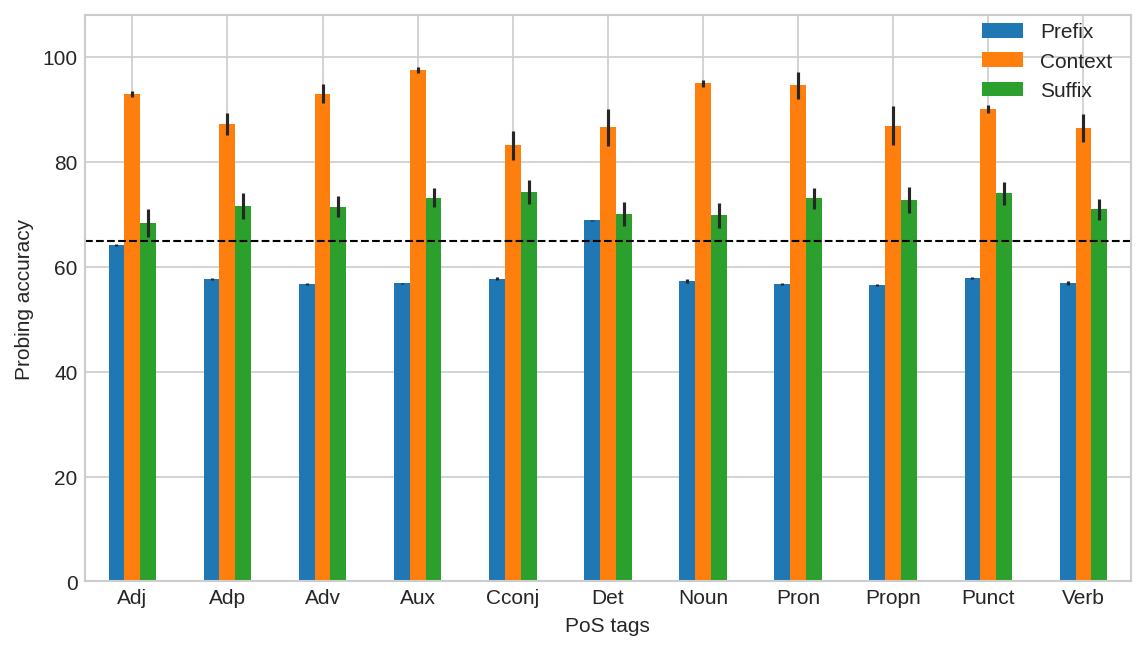
\includegraphics[width=\columnwidth]{figures/probing-all.png}
\caption{Probing accuracy based on tokens PoS tags and their positions in the sentences, from left to right: \emph{prefix}, \emph{context}, \emph{suffix}   }\label{tab:res_per_PoS}
\end{figure}

\begin{table}[ht]
  \centering
  \scalebox{0.85}{
  \begin{tabular}{lcccc}
    \toprule
    
    \multicolumn{5}{l}{\textit{Subject-verb across object relative}}\\
        Subsets &  \makecell{Mask \emph{context} tokens  \\ except \texttt{cue que} }  & Mask \texttt{cue} &Mask \texttt{que}& Mask \texttt{cue$\oplus$que} \\
    \phantom{ab} Overall    & 16.7$_{\pm 0.7}$ & 10.6$_{\pm 1.3}$ & 2.6$_{\pm 0.3}$& 13.5$_{\pm 0.6}$  \\\cline{1-5}
    \phantom{ab} 5 heuristics & 5.0$_{\pm 0.5}$&2.4$_{\pm 0.4}$&0.5$_{\pm 0.1}$&4.0$_{\pm 0.3}$\\
    \phantom{ab} 4 heuristics &15.3$_{\pm 1.0}$&10.1$_{\pm 1.6}$&3.0$_{\pm 0.4}$&12.5$_{\pm 0.6}$ \\
    \phantom{ab} 3 heuristics &28.1$_{\pm 0.8}$&19.8$_{\pm 3.0}$&5.7$_{\pm 0.4}$&24.3$_{\pm 1.1}$\\
    \phantom{ab} 2 heuristics &44.1$_{\pm 1.4}$&21.1$_{\pm 3.2}$&7.0$_{\pm 0.8}$&35.4$_{\pm 1.3}$\\
    \phantom{ab} 1 heuristics &44.7$_{\pm 1.9}$&25.3$_{\pm 2.3}$&3.2$_{\pm 0.6}$&30.8$_{\pm 1.9}$\\
    \phantom{ab} 0 heuristics &42.6$_{\pm 2.0}$&31.1$_{\pm 1.9}$&6.7$_{\pm 1.0}$&34.3$_{\pm 1.9}$\\
     \midrule
    
    \multicolumn{5}{l}{\textit{Object-past participle}} \\

    \midrule
    
    \phantom{ab} Overall      & 8.4$_{\pm 1.0}$ & 25.6$_{\pm 0.8}$  &17.9$_{\pm 0.5}$ &30.1$_{\pm 0.3}$ \\\cline{1-5}
    \phantom{ab} 5 heuristics  & 3.6$_{\pm 0.1}$& 7.8 $_{\pm 0.3}$&6.7$_{\pm 0.2}$ & 10.5$_{\pm 0.5}$\\
    \phantom{ab} 4 heuristics &7.9$_{\pm 1.1}$ & 24.0$_{\pm 0.7}$ & 15.3$_{\pm 0.4}$&27.6$_{\pm 0.4}$\\
    \phantom{ab} 3 heuristics &11.6$_{\pm 1.7}$&24.8$_{\pm 1.4}$&19.4$_{\pm 1.0}$&28.5$_{\pm 0.4}$\\ 
    \phantom{ab} 2 heuristics &12.6$_{\pm 3.3}$&40.5$_{\pm 1.6}$&39.8$_{\pm 1.4}$&53.8$_{\pm 0.5}$\\
    \phantom{ab} 1 heuristic &15.8$_{\pm 3.3}$&67.5$_{\pm 1.4}$&57.7$_{\pm 1.0}$&80.7$_{\pm 0.4}$ \\
    \phantom{ab} 0 heuristic&24.0$_{\pm 3.4}$&59.0$_{\pm 3.1}$&64.0$_{\pm 1.1}$&88.4$_{\pm 1.3}$\\
   
    
    \bottomrule
  \end{tabular}}
  \caption{Average causal effect of interventions on Transformer's NA task performance, quantified by \textbf{drop} in accuracy before and after different interventions, and further broken down based on prediction difficulty measured by the number of heuristics. The term \emph{cue} here refers to the antecedent and its modifiers (determiners and adjectives) in O-PP agreement, and to the subject and its modifiers in S-V agreement.}
    \label{tab:full_causal_res}
\end{table}

\begin{table}[ht]
  \centering
  \begin{tabular}{llcc}
    \toprule
    \multicolumn{2}{l}{Constructions}  &$\mathcal{M}$ & $\mathcal{M}_{NoPos}$ \\
    \midrule
    \multicolumn{2}{l}{Perplexity}   & 27.0   & 27.4   \\
    \midrule
    \multicolumn{4}{l}{\textit{S-V agreement}} \\
    \phantom{ab} & overall  & 98.9\%$_{\pm 0.04}$   & 98.8\% $_{\pm 0.1}$ \\\cline{2-4}
    \phantom{ab} & 5 heuristics  &99.6\% $_{\pm 0.05}$ & 99.6\% $_{\pm 0.1}$ \\
    \phantom{ab} & 4 heuristics  &99.0\% $_{\pm 0.1}$ & 98.5\% $_{\pm 0.2}$ \\
    \phantom{ab} & 3 heuristics  & 98.4\% $_{\pm 0.1}$ & 98.1\% $_{\pm 0.2}$\\
    \phantom{ab} & 2 heuristics  & 97.7\% $_{\pm 0.1}$& 97.6\% $_{\pm 0.1}$\\    
    \phantom{ab} & 1 heuristic &96.8\% $_{\pm 0.1}$& 97.2\% $_{\pm 0.2}$\\
    \phantom{ab} & 0 heuristic &94.1\% $_{\pm 0.5}$ & 94.8\% $_{\pm 0.7}$\\
    \midrule
    \multicolumn{4}{l}{\textit{O-PP agreement}} \\
     & overall  & 94.6\% $_{\pm 0.2}$  & 94.3\% $_{\pm 0.3}$     \\\cline{2-4}
      & 5 heuristics  &99.2\% $_{\pm 0.1}$ & 99.0\% $_{\pm 0.1}$ \\
     & 4 heuristics  &96.5\% $_{\pm 0.1}$ & 95.9\% $_{\pm 0.2}$\\
     & 3 heuristics  & 91.6\% $_{\pm 0.4}$& 91.3\% $_{\pm 0.6}$\\
     & 2 heuristics  & 87.6\% $_{\pm 0.4}$& 87.5\% $_{\pm 0.6}$\\    
     & 1 heuristic &77.9\% $_{\pm 0.8}$& 78.1\%  $_{\pm 1.0}$ \\
     & 0 heuristic  &76.1\% $_{\pm 1.0}$& 75.6\% $_{\pm 1.3}$\\
    \bottomrule
  \end{tabular}
\caption{Autoregressive Transformer LM's accuracy on two NA tasks with and without positional embeddings. \label{tab:TM_nopos}
}
\end{table}

\begin{table}[ht]
  \centering
  \begin{tabular}{llcc}
    \toprule
    \multicolumn{2}{l}{Constructions}  &$\mathcal{M}^{MLM}$ & $\mathcal{M}_{NoPos}^{MLM}$ \\
    \midrule
    \multicolumn{4}{l}{\textit{S-V agreement}} \\
    \phantom{ab} & overall  & 99.3$_{\pm 0.2}$   & 84.9 $_{\pm 0.8}$ \\\cline{2-4}
    \phantom{ab} & 5 heuristics  &99.7 $_{\pm 0.1}$ & 96.7 $_{\pm 0.1}$ \\
    \phantom{ab} & 4 heuristics  &99.3 $_{\pm 0.1}$ & 87.3 $_{\pm 0.3}$ \\
    \phantom{ab} & 3 heuristics  & 99.0 $_{\pm 0.2}$ & 77.1 $_{\pm 0.5}$\\
    \phantom{ab} & 2 heuristics  & 98.6 $_{\pm 0.1}$& 60.1 $_{\pm 1.1}$\\    
    \phantom{ab} & 1 heuristic &98.1 $_{\pm 0.3}$& 46.5 $_{\pm 2.1}$\\
    \phantom{ab} & 0 heuristic &95.5 $_{\pm 0.3}$ & 29.4 $_{\pm 1.8}$\\
    \midrule
    \multicolumn{4}{l}{\textit{O-PP agreement}} \\
     & overall  & 95.1 $_{\pm 0.2}$  & 72.5 $_{\pm 2.3}$     \\\cline{2-4}
      & 5 heuristics  &99.4 $_{\pm 0.05}$ & 92.2 $_{\pm 0.1}$ \\
     & 4 heuristics  &96.7 $_{\pm 0.1}$ & 79.3 $_{\pm 0.7}$\\
     & 3 heuristics  & 92.2 $_{\pm 0.3}$& 55.6 $_{\pm 1.6}$\\
     & 2 heuristics  & 88.4 $_{\pm 0.5}$& 35.4 $_{\pm 1.8}$\\    
     & 1 heuristic &82.2 $_{\pm 0.7}$& 30.3  $_{\pm 4.1}$ \\
     & 0 heuristic  &75.1 $_{\pm 1.1}$& 22.1 $_{\pm 2.5}$\\
    \bottomrule
  \end{tabular}
\caption{Masked Transformer LM's accuracy on two NA tasks with and without positional embeddings. \label{tab:MLM_nopos}
}
\end{table}

\clearpage

\customsection{Grammar and sampling details} \label{app:dataset-generation}

SLOG expands upon the COGS vocabulary, which consists of 503 nouns and 113 verbs, to additionally include \textit{wh}-words (\textit{who, what}) and \textit{that} used as a relative pronoun. In SLOG, for the sake of simplicity, we only consider restrictive relative clauses introduced by \textit{that} regardless of the animacy of the head NPs. For indirect object-extracted instances, we use the preposition stranding structure, such as \textit{the boy that Emma give a cake to}, rather than \textit{the boy to whom Emma gave a cake}.

The dataset includes the 30,000 examples from the initial COGS training set, and new examples that fall into one of the following categories: 
\begin{itemize}[itemsep=0pt, parsep=0pt, topsep=0pt]
    \item Relative clauses within object NPs, equal in number to instances with PP modifications
    \item Subject and object \emph{wh}-questions matching the quantity of their corresponding declarative sentences
    \item An equal number of four-level-nesting recursion constructions as the depth-2 instances in initial COGS
    \item A primitive example for each ditransitive verbs and verbs accepting complement clause (CP) arguments
\end{itemize}

\noindent Finally, the SLOG sampling process excludes sentences with duplicate nouns (e.g. \textit{Emma saw Emma.}).

\customsection{SLOG Full results and additional analyses} \label{sec:analysis_case}

We report the full results of the experiments discussed in Section~\ref{sec:slog_res} in Table~\ref{tab:res_cases}.

\customsubsection{Effect of the reformatted exact-match metric}
\label{app:metric}
All models exhibit higher overall accuracy with the reformatted exact-match evaluation compared to the initial metric, notably pretrained models with an over 10 percentage point increase (Table~\ref{tab:res_cases}). This suggests that the initial exact-match metric may have underestimated model performance.

\begin{table}[ht]
    \centering
    \scalebox{0.75}{
    \begin{tabular}{lccccccc}
    \toprule
    Generalization cases & \multicolumn{2}{c}{ \makecell[c]{Vanilla \\ Transformer}} & \multicolumn{2}{c}{T5}  & \multicolumn{2}{c}{LLaMa}  & AM-Parser \\
    \midrule
    Deeper PP recursion &\exactmatch{13.1$_{\pm 1.5}$} &13.1$_{\pm 1.5}$ &\exactmatch{15.7$_{\pm 0.7}$}&16.6$_{\pm 1.0}$ &\exactmatch{19.8$_{\pm 1.1}$}&20.6$_{\pm 1.0}$ &100.0$_{\pm 0.0}$ \\
    Deeper tail CP recursion &\exactmatch{0.2$_{\pm 0.1}$} &0.9$_{\pm 0.3}$ &\exactmatch{0.8$_{\pm 0.2}$}&5.3$_{\pm 0.4}$ &\exactmatch{3.9$_{\pm 0.4}$} & 12.1$_{\pm 0.7}$&100.0$_{\pm 0.0}$ \\
    Deeper center embedding &\exactmatch{0.0$_{\pm 0.0}$}& 0.0$_{\pm 0.0}$ &\exactmatch{0.0$_{\pm 0.0}$}&0.0$_{\pm 0.0}$ &\exactmatch{0.0$_{\pm 0.0}$}& 0.0$_{\pm 0.0}$&99.5$_{\pm 0.4}$ \\
     Shallower PP recursion& \exactmatch{98.7$_{\pm 0.8}$} & 98.7$_{\pm 0.8}$& \exactmatch{90.2$_{\pm 2.2}$}&93.1$_{\pm 1.9}$ & \exactmatch{97.3$_{\pm 0.9}$}&98.9$_{\pm 0.6}$ &100.0$_{\pm 0.0}$ \\
    Shallower tail CP recursion & \exactmatch{32.6$_{\pm 3.6}$} &55.2$_{\pm 4.2}$ &\exactmatch{44.8$_{\pm 2.8}$}&60.9$_{\pm 2.1}$ &\exactmatch{85.4$_{\pm 3.6}$} & 98.1$_{\pm 0.7}$&100.0$_{\pm 0.0}$ \\
    Shallower center embedding &\exactmatch{0.0$_{\pm 0.0}$} &0.0$_{\pm 0.0}$ &\exactmatch{0.0$_{\pm 0.0}$}&64.1$_{\pm 19.1}$ &\exactmatch{0.0$_{\pm 0.0}$}&50.7$_{\pm 5.7}$ &100.0$_{\pm 0.0}$ \\
    
    \midrule
    PP in subject NPs & \exactmatch{0.0$_{\pm 0.0}$} &0.0$_{\pm 0.0}$ &\exactmatch{0.0$_{\pm 0.0}$}& 0.8$_{\pm 0.5}$&\exactmatch{12.3$_{\pm 4.4}$}& 28.9$_{\pm 3.5}$& 57.6$_{\pm 8.1}$ \\
    PP in indirect object NPs &\exactmatch{42.5$_{\pm 2.2}$}& 42.5$_{\pm 2.2}$ &\exactmatch{50.1$_{\pm 1.7}$}& 53.8$_{\pm 1.4}$&\exactmatch{55.0$_{\pm 3.9}$}& 71.2$_{\pm 4.2}$ &90.4$_{\pm 8.1}$ \\
    RC in subject NPs & \exactmatch{0.0$_{\pm 0.0}$} &0.0$_{\pm 0.0}$ &\exactmatch{0.0$_{\pm 0.0}$}&0.2$_{\pm 0.2}$ &\exactmatch{3.4$_{\pm 1.6}$}& 29.5$_{\pm 3.4}$ &55.8$_{\pm 8.4}$ \\
    RC in indirect object NPs &\exactmatch{34.4$_{\pm 6.0}$}& 34.8$_{\pm 6.1}$ &\exactmatch{35.1$_{\pm 1.9}$}&36.6$_{\pm 2.1}$ &\exactmatch{48.6$_{\pm 1.9}$}& 55.0$_{\pm 2.1}$ &74.4$_{\pm 6.4}$ \\
    \midrule
    Indirect object-extracted RC &\exactmatch{4.7$_{\pm 5.6}$} &4.7$_{\pm 5.7}$ &\exactmatch{0.0$_{\pm 0.0}$}&0.0$_{\pm 0.0}$ &\exactmatch{0.1$_{\pm 0.3}$}& 2.5$_{\pm 3.2}$ &0.0$_{\pm 0.0}$ \\
    Indirect object \textit{wh}-questions  & \exactmatch{35.9$_{\pm 8.3}$}&42.4$_{\pm 13.5}$ &\exactmatch{0.0$_{\pm 0.0}$}&0.4$_{\pm 0.7}$ &\exactmatch{27.9$_{\pm 9.3}$} &73.5$_{\pm 18.4}$ & 41.4$_{\pm 42.4}$ \\
    \midrule
    Active subject \textit{wh}-questions &\exactmatch{96.7$_{\pm 2.6}$}& 97.1$_{\pm 2.4}$ &\exactmatch{90.5$_{\pm 4.0}$}&98.1$_{\pm 1.7}$&\exactmatch{92.8$_{\pm 6.4}$}& 93.3$_{\pm 6.0}$ &99.8$_{\pm 0.6}$ \\
    Passive subject \textit{wh}-questions &\exactmatch{27.4$_{\pm 1.7}$}& 31.9$_{\pm 5.4}$ &\exactmatch{20.3$_{\pm 3.8}$}&100.0$_{\pm 0.0}$ &\exactmatch{4.8$_{\pm 4.5}$}& 15.3$_{\pm 17.5}$ &100.0$_{\pm 0.1}$ \\
    Direct object \textit{wh}-questions &\exactmatch{2.8$_{\pm 3.4}$} &16.0$_{\pm 12}$ &\exactmatch{47.2$_{\pm 1.0}$}&98.5$_{\pm 0.9}$ &\exactmatch{0.5$_{\pm 0.5}$}& 8.6$_{\pm 5.7}$ &29.4$_{\pm 33.5}$ \\
    \textit{Wh}-questions with modified NPs &\exactmatch{17.6$_{\pm 0.9}$}& 17.8$_{\pm 1.3}$ &\exactmatch{20.5$_{\pm 1.0}$}&36.8$_{\pm 0.4}$ &\exactmatch{15.8$_{\pm 0.6}$}& 20.8$_{\pm 2.4}$ &55.6$_{\pm 12.5}$ \\
    \textit{Wh}-questions long movement &\exactmatch{4.0$_{\pm 7.8}$}& 4.9$_{\pm 9.5}$ &\exactmatch{23.3$_{\pm 4.3}$}&24.9$_{\pm 5.1}$ &\exactmatch{0.8$_{\pm 1.4}$}&3.0$_{\pm 4.7}$ & 0.0$_{\pm 0.0}$ \\
    \midrule
    
   
    \textbf{Overall} &\textbf{\exactmatch{24.2$_{\pm 1.0}$}}& \textbf{27.1$_{\pm 2.0}$} &\textbf{\exactmatch{23.4$_{\pm 1.1}$}}&\textbf{40.6$_{\pm 1.0}$} &\textbf{\exactmatch{27.6$_{\pm 1.0}$}}& \textbf{40.1$_{\pm 1.8}$}&  \textbf{70.8$_{\pm 4.3}$} \\
    
    \bottomrule
    \end{tabular}}
    \caption{Mean accuracy (\%) using exact-match is shown in gray, accuracy using reformatted exact-match described in Section~\ref{sec:slog_ex_setup} is shown in black. AM-Parser's graph-based output yields identical scores for both metrics hence only a single column is reported.
    }
    \label{tab:res_cases}
\end{table}

\customsubsection{RC Modifiers in unseen positions} \label{app:RC_modifiers_results}
\begin{table}[t]
    \centering
    \scalebox{0.8}{
    \begin{tabular}{lccccc}
      \toprule
       Generalization cases & \makecell[c]{Long pred-arg \\dependency?} & \makecell[c]{Vanilla \\Transformer} & T5 & LLaMa&\makecell[c]{AM \\parser}   \\
       \midrule
       \makecell[l]{ {\scriptsize Sub-case: Passive indirect objects} \\  \textbf{A fish} \textbf{was given} to  [ a cat that slept ]$_{\textcolor{blue}{\bf iobj}}$. } & \ding{55}  & 72.0$_{\pm 6.6}$  & 74.2$_{\pm 2.7}$   &97.1$_{\pm 1.2}$ & 99.5$_{\pm 0.6}$ \\
       \makecell[l]{ {\scriptsize Sub-case: Indirect object in PP datives  } \\   Emma \textbf{gave a fish} to  [ a cat that slept ]$_{\textcolor{blue}{\bf iobj}}$.} & \ding{55} & 27.0$_{\pm 9.8}$  & 38.9$_{\pm 5.3}$   &72.7$_{\pm 7.8}$ & 99.3$_{\pm 1.1}$  \\
      \makecell[l]{ {\scriptsize Sub-case: Indirect object in double object datives} \\    Emma \textbf{gave} [ a cat that slept ]$_{\textcolor{blue}{\bf iobj}}$ \textbf{a fish}.} & \ding{51} & 7.9$_{\pm 8.5}$ & 0.2$_{\pm 0.2}$   &0.3$_{\pm 0.3}$& 28.9$_{\pm 17.2}$ \\
      \makecell[l]{ {\scriptsize Subject} \\ \  [\textbf{A cat} that slept]$_{\textcolor{blue}{\bf subj}}$ \textbf{ate} a fish. } & \ding{51} & 0.0$_{\pm 0}$ & 0.2$_{\pm 0.2}$ &29.4$_{\pm 3.4}$&51.7$_{\pm 8.4}$\\
      \bottomrule
    \end{tabular}    
    }
    \caption{Performance of RC modification generalization broken down by construction.} 
    \label{tab:cat_1_RC_analysis}
\end{table}

Generalizing RC modifiers to unseen positions presents a similar challenge as PP modification cases, due to unobserved long-distance dependencies. As shown in Table \ref{tab:cat_1_RC_analysis}, all models exhibit a significant performance discrepancy between constructions involving unseen long predicate-argument dependencies and those that do not.

For novel positions that introduce long predicate-argument dependencies, RC modification in the indirect object appears more difficult than in the subject position, contrary to the case with PP modifiers. The primary error pattern (\ref{ex:iobj_RC_error}) demonstrates that models struggle to detect the RC boundary when the relative clause ends with a verb. They systematically misinterpret the indirect object \texttt{a fish} of the main verb \texttt{gave} as the direct object of the adjacent embedded verb \texttt{slept}.  

\customsubsection{Passive subject \emph{wh}-questions} \label{app:subj_q}
For subject \emph{wh}-questions, which exhibit no gap, T5 and AM-Parser perform near-perfectly on both active and passive subject questions. Vanilla Transformer and LLaMa also perform well on active subject questions, but achieve much lower performance on passive subject questions. This performance discrepancy is the most evident in sub-cases where passive subjects function as theme (e.g., (\ref{ex:subj_q_input}))---the vanilla Transformer has near-zero accuracy for these sub-cases, systematically failing to map \emph{wh}-words to `?' as in (\ref{ex:subj_q_error}):  

\begin{exe}
\ex \label{ex:subj_q_input}Input: What was eaten by Emma ?
\begin{xlist}
    \ex \label{ex:subj_q_gold} Gold:  \lform{eat.theme (x$_2$, ?) $\land$ eat.agent (x$_2$, Emma)}
    \ex \label{ex:subj_q_error} Output of Vanilla Transformer and LLaMa:  \lform{eat.theme (x$_2$,  \textcolor{red}{x$_4$}) $\land$ eat.agent (x$_2$, Emma)}
\end{xlist}
\end{exe}

\noindent As discussed in Section~\ref{subsec:am_parser_analysis}, this error pattern may result from the highly imbalanced label distribution in training output space. Both LLaMa and vanilla Transformer are inclined to repeat the substantially more common subsequence \lform{theme($x_i,x_j$)} over \lform{theme($x_i$,?)}. 

 \begin{exe}
\ex \label{ex:iobj_RC_error} Gold LF and model-predicted LF for \textit{Emma gave a cat that slept a fish}:
    \begin{xlist}
        \small{
        \ex \label{ex:iobj_a_dobj_gold_RC} Gold: \lform{give.agent ($x_1$,Emma) $\land$ give.\textbf{recipient} ($x_1,x_3)$ $\land$  give.theme ($x_1,x_7$)$\land$ cat($x_3$) $\land$ cat.nmod (x$_3,x_5$) $\land$ sleep.agent($x_5,x_3$) $\land$ fish($x_7$)}
    \ex \label{ex:iobj_a_dobj_pred_RC} Out: \lform{give.agent ($x_1$,Emma) $\land$ give.\textcolor{red}{theme} ($x_1,x_3)$ $\land$  cat($x_3$) $\land$ cat.nmod (x$_3,x_5$) sleep.agent($x_5,x_3$) $\land$ \textcolor{red}{sleep.theme($x_5,x_7$)} $\land$fish($x_7$) }
    }
    \end{xlist}
\end{exe}

\customsubsection{\emph{Wh}-questions with modified NPs} 
In \emph{wh}-questions with PP and RC modifiers, even though the SLOG training set only contains \emph{wh}-questions with unmodified NPs, all models generalize well (accuracy > 80\%) to direct object NPs with modifiers (e.g., \textit{Who ate a cake on the table?}). These are cases where the modification pattern is observed in training as a part of declarative sentences. In contrast, performance declines when models encounter \emph{wh}-questions with modifiers in the indirect object position (i.e., modification structure not observed as part of declarative sentences). Similarly, for \emph{wh}-questions with subject position modifiers, the performance is very low: both T5 and vanilla Transformers achieve near-zero accuracy, and LLaMa achieves around 5\%.

This observation mirrors the patterns discussed in \S\ref{subsec:long_distance_hard}, attributed to difficulties introduced by unseen subject-verb dependencies across PPs or RCs. In contrast, the structure-aware model exhibits significantly better performance in \textit{wh}-question with subject modification.

\customsection{SLOG: Results of variable-free LFs} \label{app:varfree_res}
\begin{table}[ht]
    \centering
    \begin{tabular}{lcccc}
    \toprule
    Generalization cases & \makecell[c]{Vanilla \\ Transformer} & T5  & LLaMa  \\
    \midrule
    Deeper PP recursion & 7.8$_{\pm 1.8}$ & 63.0$_{\pm 2.9}$ & 90.9$_{\pm 3.3}$ \\
    Deeper tail CP recursion & 1.0$_{\pm 0.5}$ & 46.2$_{\pm 2.6}$ & 44.1$_{\pm 7.9}$ \\
    Deeper center-embedding & 0.0$_{\pm 0.0}$ & 7.8$_{\pm 1.1}$ & 9.4$_{\pm 2}$ \\
    Shallower PP recursion & 98.2$_{\pm 1.6}$ & 99.6$_{\pm 0.9}$ & 100.0$_{\pm 0.0}$ \\
    Shallower tail CP recursion & 89.3$_{\pm 3.3}$ & 99.3$_{\pm 1.6}$ & 100.0$_{\pm 0.0}$ \\
    Shallower center-embedding & 0.1$_{\pm 0.2}$ & 99.8$_{\pm 0.3}$ & 99.8$_{\pm 0.4}$ \\

    \midrule
    PP in subject NPs & 0.2$_{\pm 0.3}$ & 73.2$_{\pm 9.0}$ & 93.4$_{\pm 4.8}$ \\
    PP in indirect object NPs & 29.3$_{\pm 10.7}$ & 97.4$_{\pm 2.1}$ & 98.1$_{\pm 1.9}$ \\
    RC in subject NPs & 0.1$_{\pm 0.1}$ & 60.8$_{\pm 6.3}$ & 73.9$_{\pm 13.5}$ \\
    RC in indirect object NPs & 4.0$_{\pm 1.9}$ & 71.9$_{\pm 0.8}$ & 73.6$_{\pm 3.9}$ \\
    \midrule
    Indirect object-extracted RC & 0.0$_{\pm 0.0}$ & 62.4$_{\pm 7.5}$ & 3.3$_{\pm 2.8}$ \\
    Indirect object \textit{wh}-questions & 34.1$_{\pm 31.1}$ & 93.4$_{\pm 4.8}$ & 83.8$_{\pm 11.3}$ \\
    \midrule
    Active subject \textit{wh}-questions & 99.0$_{\pm 0.5}$ & 99.8$_{\pm 0.3}$ & 96.2$_{\pm 2.6}$ \\
    Passive subject \textit{wh}-questions & 57.3$_{\pm 23.8}$ & 99.9$_{\pm 0.1}$ & 96.0$_{\pm 3.0}$ \\
    Direct object \textit{wh}-questions & 41.8$_{\pm 3.8}$ & 48.4$_{\pm 0.4}$ & 44.1$_{\pm 4.6}$ \\
    \textit{Wh}-questions with modified NPs & 18.1$_{\pm 2.3}$ & 68.0$_{\pm 1.9}$ & 69.4$_{\pm 6.8}$ \\
    \textit{Wh}-questions long movement & 7.4$_{\pm 3.7}$ & 45.6$_{\pm 4.6}$ & 35.7$_{\pm 6.5}$ \\
    \midrule
    Total & 28.7$_{\pm 4.1}$ & 72.7$_{\pm 1.1}$ & 71.3$_{\pm 3}$ \\
    \bottomrule
    \end{tabular}
    \caption{Mean accuracy (\%) on SLOG using the variable-free logical form of \citet{qiu-etal-2022-improving}.}
    \label{tab:res_cases_varfree}
\end{table}

Table~\ref{tab:res_cases_varfree} reports the accuracy on SLOG using variable-free logical forms. The AM-Parser is unable to handle the variable-free format and therefore is omitted. The hyperparameters for the three tested models are the same as the experiments described in Section~\ref{sec:slog_ex_setup}.

The variable-free LF, as discussed in Section~\ref{sec:data_generation} and \citet{wu2023recogs}, exhibits certain limitations and ambiguities which render direct comparisons with variable-based LF results inappropriate. Regardless, all three models achieve higher accuracy scores on the variable-free LFs compared to the COGS LFs, with pretrained models experiencing a particularly significant boost. This aligns with the observations of \citealt{qiu-etal-2022-evaluating}. 

Despite the change in LF, the overall trends and challenges remain consistent. The vanilla Transformer struggles with the same generalization cases, failing to extrapolate to deeper recursion depths and struggling with cases involving unseen long-distance dependencies. Pretrained models, while exhibiting better overall performance, continue to struggle with more structurally complex generalization cases in their respective categories. These include deeper center-embedding, indirect object-extracted RC and \emph{wh}-questions with long movement.



\customsection{Discussion and limitations}

While SLOG offers a targeted and well-controlled approach to assess structural generalization, it presents some limitations.

First, SLOG is a synthetic corpus and covers only a fraction of the diverse structures in English. Furthermore, previous research has demonstrated that the design of \ac{MR} can have a nontrivial effect on model performance in semantic parsing tasks \citep{guo-etal-2019-towards,herzig2021unlocking,qiu-etal-2022-evaluating}. For example, as noted by \citet{wu2023recogs}, the variable indexing scheme may introduce additional semantically irrelevant challenges when assessing structural generalization. SLOG's reformatted exact-match evaluation metric partially addresses this concern by taking into consideration several variations of MRs that are semantically equivalent including MRs that are equivalent up to constant renaming. However, a more comprehensive study of the effect of artifacts from the formalism is left to future work. 

Second, there also exist challenges specific to the evaluation of pretrained models. That is, distributional shift between training and generalization sets intended by SLOG, such as withholding the constructions \textit{PPs modifying subject NPs} from training, is difficult to strictly enforce when pretraining is involved \cite{kim2022uncontrolled}. This potential violation of distributional control makes the interpretation of the obtained results difficult; we cannot disentangle whether generalization success in pretrained models derives from genuine compositional capabilities or simply exposure during pretraining to the target constructions meant to be withheld from the evaluated models. Still, corpus analyses such as \citet{karlsson2007constraints} suggest that deep center-embedding beyond three levels is very rare in naturally occurring data, so it is possible that very deep embedded structures are withheld as intended even from models exposed to large amounts of pretraining data. We hope the additional structural generalization cases that SLOG offers can also help with future work investigating the interaction between structures available in pretraining data and structural generalization.